\section{}
\[
H(s)=\frac{10}{s+10}\,.
\]
\subsection{Bode-Diagramm}
\begin{center}
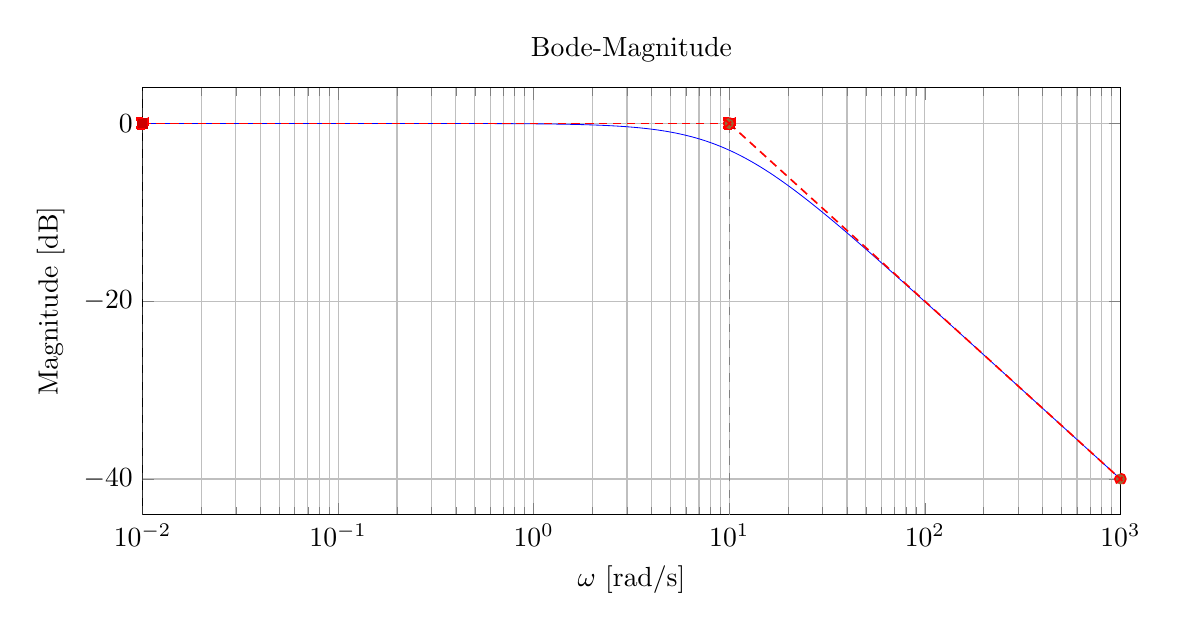
\begin{tikzpicture}
\begin{semilogxaxis}[
  width=14cm,height=7cm,
  xmin=1e-2,xmax=1e3,
  xlabel={$\omega$ [rad/s]},
  ylabel={Magnitude [dB]},
  grid=both,
  ytick distance=20, 
  title={Bode-Magnitude}
]
\addplot[
  domain=1e-2:1e3,
  samples=600,
  mark=none,
  line width=0.3pt,
  blue
] {-20*ln(sqrt(1 + (x/10)^2))/ln(10)};
\addplot+[domain=1e-2:1e1,samples=2,dashed,dash pattern=on 3pt off 2pt,line width=0.6pt,red] {0};
\addplot+[domain=1e1:1e3,samples=2,dashed,dash pattern=on 3pt off 2pt,line width=0.6pt,red] {-20*ln(x/10)/ln(10)};
\draw[gray,dashed] (rel axis cs:0,0) -- (rel axis cs:0,1);
\draw[gray,dashed] (axis cs:10,\pgfkeysvalueof{/pgfplots/ymin}) -- (axis cs:10,\pgfkeysvalueof{/pgfplots/ymax});
\node[gray,anchor=south east] at (axis cs:10,\pgfkeysvalueof{/pgfplots/ymax}) {\scriptsize Pol $\omega_p=10$};
\end{semilogxaxis}
\end{tikzpicture}
\vspace{6mm}
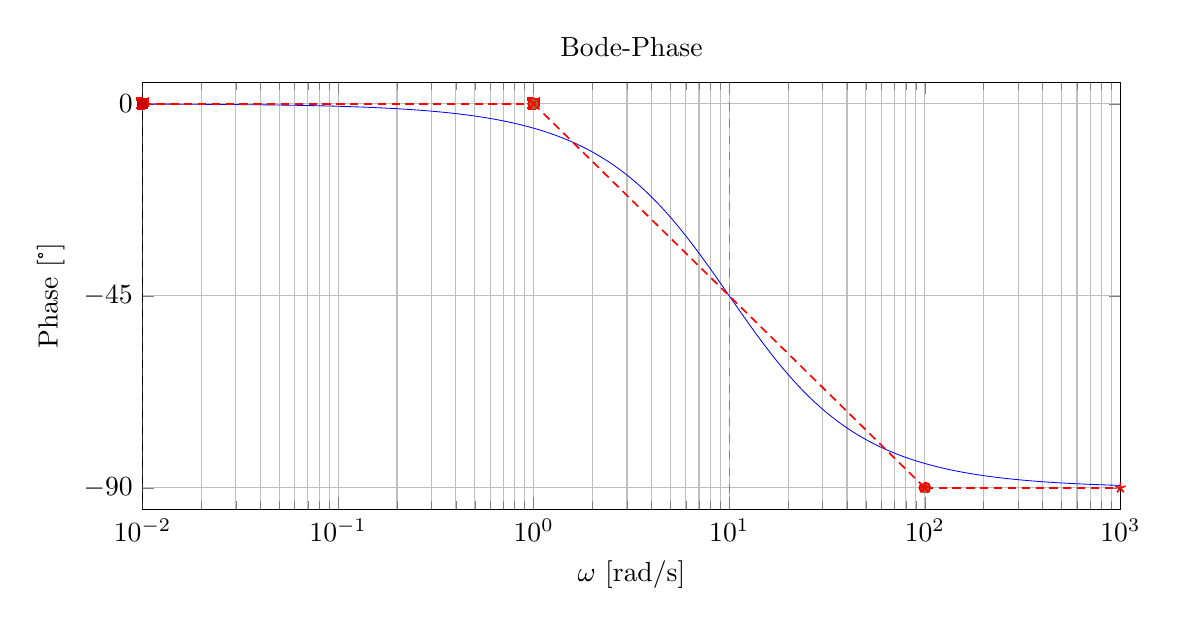
\begin{tikzpicture}
\begin{semilogxaxis}[
  width=14cm,height=7cm,
  xmin=1e-2,xmax=1e3,
  ytick distance=45,
  ymin=-95,ymax=5,
  xlabel={$\omega$ [rad/s]},
  ylabel={Phase [°]},
  grid=both,
  title={Bode-Phase}
]
\addplot[
  domain=1e-2:1e3,
  samples=600,
  mark=none,
  line width=0.3pt,
  blue
] {-atan(x/10)};
\addplot+[domain=1e-2:1e0,samples=2,dashed,dash pattern=on 3pt off 2pt,line width=0.6pt,red] {0};
\addplot+[domain=1e0:1e2,samples=2,dashed,dash pattern=on 3pt off 2pt,line width=0.6pt,red] {-45 - 45*ln(x/10)/ln(10)};
\addplot+[domain=1e2:1e3,samples=2,dashed,dash pattern=on 3pt off 2pt,line width=0.6pt,red] {-90};
\draw[gray,dashed] (rel axis cs:0,0) -- (rel axis cs:0,1);
\draw[gray,dashed] (axis cs:10,\pgfkeysvalueof{/pgfplots/ymin}) -- (axis cs:10,\pgfkeysvalueof{/pgfplots/ymax});
\node[gray,anchor=south east] at (axis cs:10,\pgfkeysvalueof{/pgfplots/ymax}) {\scriptsize Pol $\omega_p=10$};
\end{semilogxaxis}
\end{tikzpicture}
\end{center}
\newpage
\subsection{Erklärung (ausführlich)}
\begin{description}[leftmargin=1.2em,labelsep=.6em,font=\bfseries]

\item[1. Normalform herstellen.]
Bringe die Übertragungsfunktion exakt in die im Skript definierte Standardform für reelle Pol-/Nullstellen.
\[
H(s)=\frac{1}{1+sT_p}\quad\text{mit}\quad T_p=\frac{1}{10}.
\]
Hier haben wir: \[
\underline{F}_1(s)=\frac{1}{1+sT_p}\quad\text{und}\quad K_0 = 1\quad \text{und}\quad r = 0.
\]
Klassifizikation des ersten Teilglieds $\underline{F}_1$: reelles Polglied (LHP) erster Ordnung.

\item[2. Eckfrequenz bestimmen und sortieren.]
Bestimme die Eckfrequenz aus der Zeitkonstante:
\[
\omega_p=\frac{1}{T_p}=10\,\mathrm{rad/s}.
\]
Es existiert nur diese Eckfrequenz; die aufsteigende Sortierung \(\omega_1<\omega_2<\dots\) ist damit trivial. 

\item[3. Startpunkt des Amplitudengangs festlegen (Geradennäherung).]
Setze die Startfrequenz gleich der kleinsten Eckfrequenz \(\omega_{\min}=\omega_p = 10\,\mathrm{rad/s}\). Verwende die Skript-Regel
\[
F_{\mathrm{dB}}(\omega_{\min})=20\log_{10}\!\Big(|K_0\,F^*_{ges}(0)|\cdot\,\omega_{\min}^{\,r}\Big) = 20 \log_{10}(1) = 0\,\mathrm{dB}.
\]
Hier gilt \(K_0=1\), \(r=0\) und \(F^*_{ges}(0)=1\Rightarrow F_{\mathrm{dB}}(\omega_{\min})=0\,\mathrm{dB}\). Dieser Punkt nützt uns als Anker für die Geradennäherung. 

\item[4. Verlauf links vom Startpunkt zeichnen.]
Für \(\omega<\omega_{\min}\) bleibt die Amplituden-Asymptote waagrecht, denn die Anfangssteigung beträgt \(r\cdot 20\,\mathrm{dB/dec}=0\). Trage also eine horizontale Linie bei \(0\,\mathrm{dB}\) ein. 

\item[5. Steigungswechsel an der Eckfrequenz eintragen.]
Ein einfaches Polglied \(1/(1+sT_p)\) reduziert die Steigung ab \(\omega_p\) um \(20\,\mathrm{dB/dec}\). Da bis jetzt die Steigung \(0\,\mathrm{dB/dec}\) betrug, ist diese ab jetzt \(-20\,\mathrm{dB/dec}\). Zeichne rechts von \(\omega_p\) die Gerade mit Steigung \(-20\,\mathrm{dB/dec}\). Die Formel für die Geradennäherung lautet:
\[
|H(j\omega)|_{\mathrm{dB}}\approx -20\log_{10}\!\Big(\frac{\omega}{10}\Big)\quad(\omega\ge 10).
\]
Mehrfachpole würden die Änderung mehrfach zählen; hier nicht nötig. 

\item[6. Eckabrundung korrekt berücksichtigen.]
Bei einfachen reellen Polen ergibt sich am Knickpunkt \(\omega=\omega_p\) eine Abweichung von \(-3\,\mathrm{dB}\) gegenüber der Gerade.
\item[7. Phasenstartwert festlegen.]
Nutze die Regel für \(\omega\to 0\): Da \(K_0F_{ges}(0)>0\) und \(r=0\), ist der Startwert der Phase
\[
\varphi(0)=r \cdot 90^\circ=0^\circ.
\]

\item[8. Phasenänderung durch das Polglied eintragen.]
Ein reelles Polglied erster Ordnung erzeugt insgesamt eine Phasenänderung von \(-90^\circ\). Trage die Näherung ein:
\[
\varphi(\omega)\approx
\begin{cases}
0^\circ,& \omega\le 0.1\,\omega_p\;(=1),\\
\text{linear mit Steigung }-45^\circ/\text{Dec},& 0.1\,\omega_p<\omega<10\,\omega_p\;(=100),\\
-90^\circ,& \omega\ge 10\,\omega_p\;(=100).
\end{cases}
\]
Das lineare Zwischenstück kann Formelkonform als \(\varphi(\omega)\approx -45^\circ-45^\circ\log_{10}(\omega/10)\) dargestellt werden (hier mit \(\omega_p=10\)). 

\item[9. Grenzwerte und Konsistenz prüfen.]
DC: \(|H(0)|=1\Rightarrow 0\,\mathrm{dB}\), \(\varphi(0)=0^\circ\). HF: \(|H(j\omega)|\sim 10/\omega\Rightarrow -20\log_{10}(\omega/10)\,\mathrm{dB}\)). Pol-/Nullzählung bestätigt die Endphase: Zählergrad \(m=0\), Nennergrad \(n=1\Rightarrow \varphi(\infty)=(m-n)\cdot 90^\circ=-90^\circ\). 

\end{description}

\subsubsection*{Stückweise Näherungen (für die Skizze)}
\[
|H(j\omega)|_{\mathrm{dB}}\approx
\begin{cases}
0,& \omega\ll 10,\\[2pt]
-10\log_{10}2,& \omega=10,\\[2pt]
-20\log_{10}(\omega/10),& \omega\gg 10,
\end{cases}
\]
\vspace{0.3cm}
\[
\varphi(\omega)\approx
\begin{cases}
0^\circ,& \omega\le 1,\\[2pt]
-45^\circ-45^\circ\log_{10}(\omega/10),& 1<\omega<100,\\[2pt]
-90^\circ,& \omega\ge 100.
\end{cases}
\]

\newpage